%!TEX root = ../thesis.tex
%*******************************************************************************
%****************************** Third Chapter **********************************
%*******************************************************************************
\chapter{Discussion}

% **************************** Define Graphics Path **************************

\graphicspath{{Chapter5/Figs/Vector/}{Chapter5/Figs/}}


\section{Non-Parametric}
Three algorithms tested of non-parametric variety producing several noticeable results. Firstly, Monte Carlo sampling outperformed both Greedy and RoD sampling. This is demonstrated convincingly through Figure~\ref{fig:nPComp} where results from the greedy results suggest the worst accuracy.

Despite the greedy algorithm demonstrating the worst accuracy, interesting results were shown with RoD sampling. Poor selection is evidently present with the first sample set, although rapid improvement quickly follows. Indeed, after the first iteration, the learning rate is superior to the other two algorithms. An extra iteration may indeed have seen RoD surpassing Monte Carlo. This is expected as the ROD algorithm specifically targets regions of the model which are challenging causing the largest changes towards proper fitting.

Both RoD and greedy sampling are suspected to suffer from clusterisation whereby data points similar to each other in the feature space are sampled within the same batch, thus reducing the total information conveyed per batch operation. This is believed to be particularly costly with the first iteration as the model will heavily overfit to the new cluster it has sampled. The random nature of Monte Carlo reduces this prospect, hence the apparent promising performance of a random sampling methodology. Evidence to this is shown in Figure~\ref{fig:MCTestSet}, Figure~\ref{fig:GreedyTestSet}, and Figure~\ref{fig:RODTestSet}.

\begin{figure}[h]
    \begin{center}
        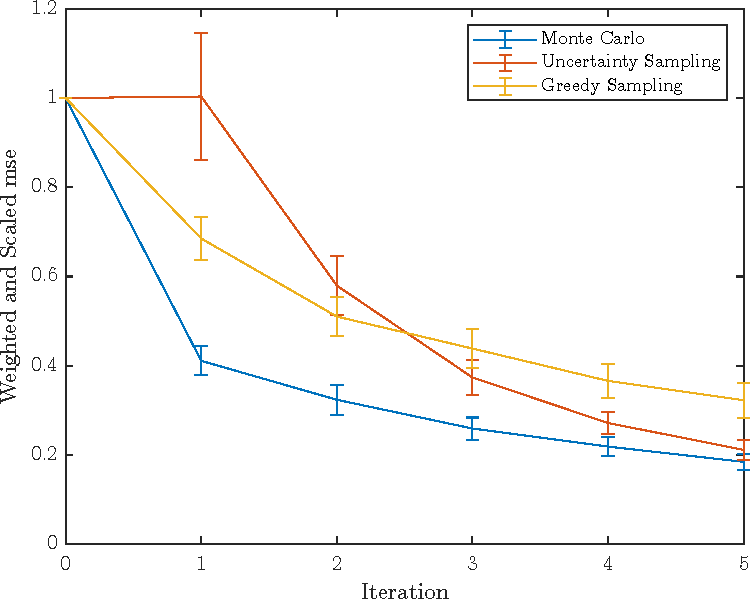
\includegraphics{nonParamComp1.pdf}
        \caption[Non-parametric comparison]{Comparison of different non-parametric algorithms with standard deviations represented as error bars.}
        \label{fig:nPComp}
    \end{center}
\end{figure}

This demonstrates a danger with Batch Active Learning. It is very easy to produce a learning algorithm which actually performs worse than random screening.

\section{Parametric}
Different classes of parametric algorithms were tested. The first of these is a first order composite algorithm, RoD with Greed: i.e. uses different active learning algorithms as a base. The second is a clustering algorithm with the number of clusters left as a parameter. The third is a second order composite active learning algorithm which combines the other two parametric functions, named RoDGer. A constant improvement is seen throughout these algorithms, with RoDGer performing the best.

\begin{figure}[h]
    \begin{center}
        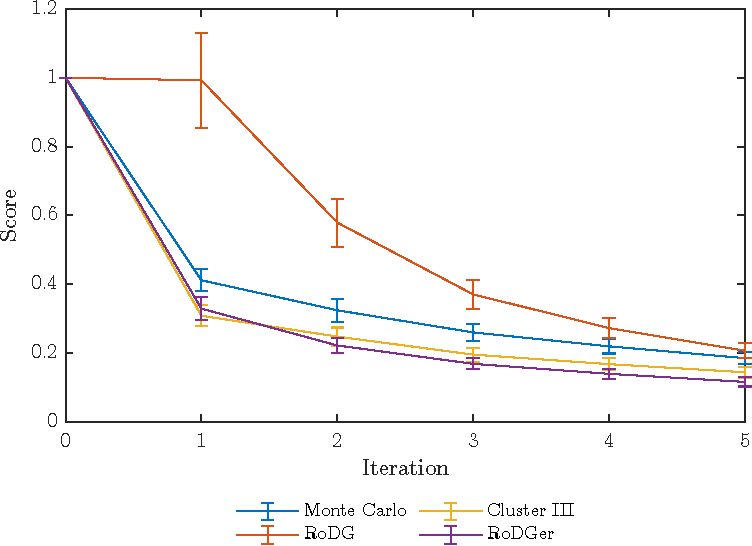
\includegraphics{paramComp1.pdf}
        \caption[Non-parametric comparison]{Comparison of different parametric algorithms with standard deviations represented as error bars.}
        \label{fig:pComp}
    \end{center}
\end{figure}

Several points of interest are highlighted with these results. Firstly, despite improving upon RoD, RoD with Greed is still beaten by Monte Carlo sampling. Again, the methodology suffers from clustering of points. This is shown with the ability of Cluster III outperforming Monte Carlo. The progression through the different cluster algorithms also sees improvement with progression, as anticipated.

The sampling process of the Cluster III algorithm demonstrates its ability at outperforming the random sampling methodology of Monte Carlo even within the first iteration. The RoDGer algorithm sacrifices some of this initial performance for longer term gain, as shown by the worse performance after the first iteration. By the second iteration, the difference becomes insignificant, with the error for each algorithm. By the end of the fifth iteration, the RoDGer algorithm convincingly outperforms the other algorithms.

Upon investigation of the parameters settled upon within these several points arise. Firstly with RoD with Greed, at low $\alpha$, the score appears uncorrelated with $\alpha$, only experiencing a significant rise with $\alpha{}>0.4$. Thus, it can be surmised that RoD is the driving force, with evidence given by the final scores for RoD and RoD with Greed algorithms arising within error of each other.

On the other hand, the sensitivity of Cluster III is extremely low to cluster size, demonstrated by Figure~\ref{fig:clusterTest}. Here, no significant change is observed within the significant parameter range. It is believed this is due to the highest ranking points remaining within the top clusters as large clusters are likely to remain the largest, even with an increased number of clusters. Thus, the top candidates are likely to remain in the same region of the feature space.

Most surprising are the parameters found for the RoDGer, shown in Figure~\ref{fig:paramHg}. Here, it appears the highest sensitivity is based on $\alpha_2$, the exponent to the RoD with Greed score. This indeed shows a difference from Rod with Greed, where the Greed aspect appeared to be borderline irrelevant, with final results within error of RoD. Comparatively, $\alpha_0$ and $\alpha_1$ appear to have a linear fit.

\begin{figure}[H]
    \begin{center}
        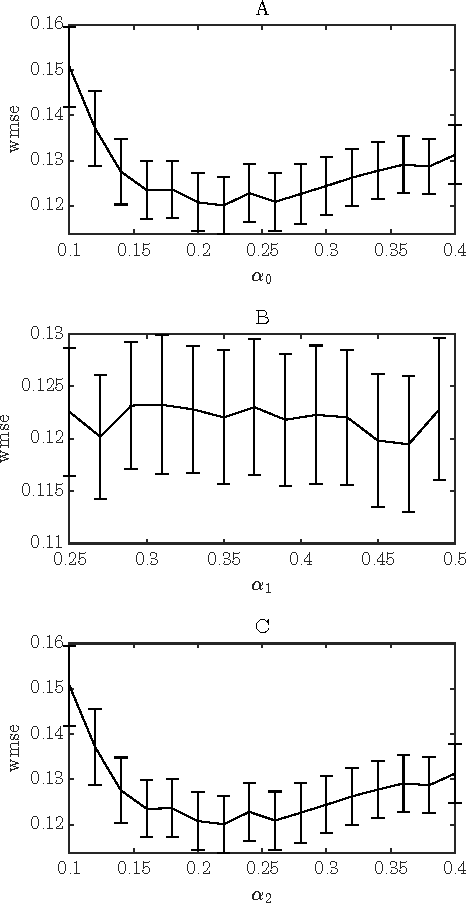
\includegraphics{hgParams.pdf}
        \caption[Non-parametric comparison]{Comparison of different parametric algorithms with standard deviations represented as error bars.}
        \label{fig:paramHg}
    \end{center}
\end{figure}

The use of curve fitting has, up until now been avoided. This is due to the difficulty in procuring the forms of these curves. Take Figure~\ref{fig:RODTestSet} where the first iteration produces no significant change. By fitting a curve, the results here could be misrepresented, so interpolation has been used in most cases to guide the eye. In Figure~\ref{fig:paramHg}, it was considered essential to present the different in form between ${\alpha_0}$, ${\alpha_1}$, and ${\alpha_2}$ so a curve has been added to guide the reader to the differences in form. Polynomial fits were used for each subfigure, with A and B using 1st order and C using 4th order.

\section{Problem Sensitivity}
The problem set up provides an estimation of a fixed number of iteration and sample size. What if these change? Are the parameters overfitted to this specific problem? If deviations from this are taken, are the intelligent methods worse than Monte Carlo? This is important to determine, as there is a significant potential cost to such an inefficiency.

Monte Carlo is tested compared to RoDGer and RoD, using the already fitted parameters where required. Monte Carlo is included to demonstrate the baseline case, while RoDGer is included due to producing the best results in previous testing. RoD has been included to assess if the learning rate maintains significantly higher than Monte Carlo in an extended testing range. Results have been presented in Figure~\ref{fig:sensi1}. Convergence of RoD to Monte Carlo is observed, with RoDGer consistently outperforming the other two algorithms.

\begin{figure}[H]
    \begin{center}
        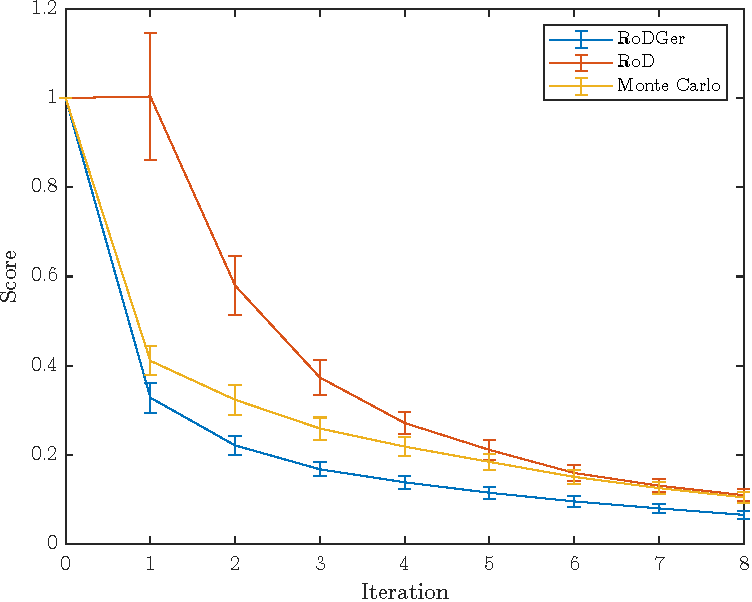
\includegraphics{Sensi1.pdf}
        \caption[Results of prolonged sampling]{Comparison of different parametric algorithms with standard deviations represented as error bars over an extended number of iterations.}
        \label{fig:sensi1}
    \end{center}
\end{figure}

Using sample sizes of 50 and 150 on Monte Carlo and RoDGer supports the power of RoDGer over simply using Monte  Carlo.

\begin{figure}[H]
    \begin{center}
        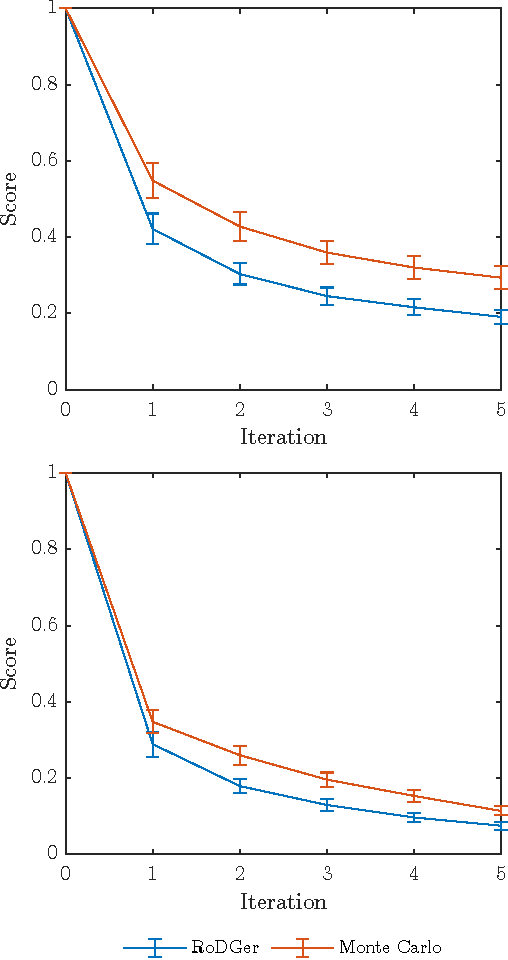
\includegraphics{Sensi2.pdf}
        \caption[Results of prolonged sampling]{Comparison of different parametric algorithms with standard deviations represented as error bars over an extended number of iterations.}
        \label{fig:sensi2}
    \end{center}
\end{figure}

Finally, an investigation into using a reduced set of models is undertaken, using Bayesian ridge, k-nearest neighbours, and a multi-layer perceptron regressor (MLPR). This last model is a neural network, chosen since it represents a different class of machine learning model. The other two were used within other trial in order to allow a sample standard deviation to be returned, as required by algorithms relying on the predict\_error method of the Model class. Results are shown in Figure~\ref{fig:modelSensi}, demonstrating the robustness of RoDGer against model changes.

\begin{figure}[H]
    \begin{center}
        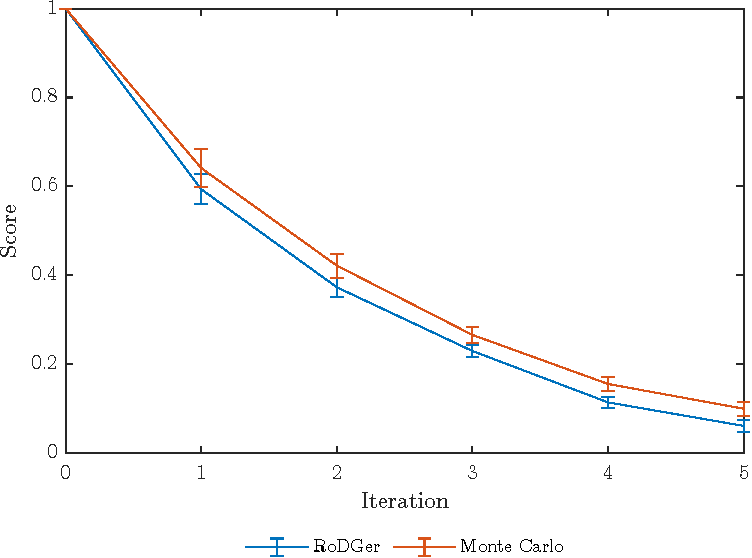
\includegraphics{Models.pdf}
        \caption[Sensitivity to Model Selection]{Comparison of different parametric algorithms with standard deviations represented as error bars over an extended number of iterations.}
        \label{fig:modelSensi}
    \end{center}
\end{figure}


\section{Refinement}
There are several points for progression that are worth discussing. Firstly, the training system requires improvement. Despite the observations of parallelisation leading to a situation of $\mathcal{O}(c)$ given an infinite number of processing units, an infinite number of processing units unfortunately do not exist. In the event of three parameters, the current methodology requires $N_\mathrm{train}\prod(n_{\alpha_i})$ executions of the learning algorithm, where $n_{\alpha_i}$ is the number of different values tested for $\alpha_i$. Even with simply 3 different values tested for each parameter in the RoDGer algorithm, this equates to $\sim{}4500$ executions of the algorithm. Thus, as the maximum number of CPUs available was 380, the training process became $\mathcal{O}\left(N_\mathrm{train}\prod{n_{\alpha_i}}\right)$. A potential solution would be segmentation, where the datasets are split into smaller groups with which are tested on a sample of the parameter space, with results from these smaller groups amalgamated at the end. Additionally, active learning could be used in the determination of the minima. Here, the goal would be to find the minima using as few parameter values as possible.

The current implementation of the scoring system is simple. Although this would please Occam's barber, it is believed that this is not satisfactory for the aggressive pursuit of effective drugs. One possibility is only scoring samples which show a pChEMBL greater than seven. This puts a greater weight on these samples, although a multidisciplinary discussion is required here. This could potentially be aided by categorising the data set instead, instead separating results into $\mathrm{pChEMBL}>7$ and $\mathrm{pChEMBL}\leq{}7$.

% Interest could be placed on parameter optimisation for each iteration

% Finally, testing on actual drugs is essential in proving the concept. 

\section{Link to Covid}
\blindtext[1]

